\documentclass{article}
\usepackage[utf8]{inputenc}
\usepackage{mathtext}
\usepackage{amsmath}
\usepackage[colorlinks=true, linkcolor=blue]{hyperref}
\usepackage[T1]{fontenc}
\usepackage[utf8]{inputenc}
\usepackage[english, bulgarian, russian]{babel}
\usepackage{tikz}
\usepackage{pgfplots}
\usepackage{indentfirst}
\usepackage[export]{adjustbox}
\usepackage{lipsum} % sample text
\usepackage{floatflt}
\usepackage{multirow}
\usepackage{geometry} 
\usepackage{animate}
\geometry{verbose,a4paper,tmargin=2cm,bmargin=2cm,lmargin=1.5cm,rmargin=1.5cm}
\setlength{\parindent}{0.65cm}
\setlength{\parskip}{0.15cm}

\usepackage{wrapfig}
\usepackage{array,graphicx,caption}


%Матеша
\usepackage{amsmath,amsfonts,amssymb,amsthm,mathtools} % AMS
\usepackage{icomma} % "Умная" запятая

%\mathtoolsset{showonlyrefs=true} % Показывать номера только у тех формул, на которые есть \eqref{} в тексте.

%% Шрифты
\usepackage{euscript}	 % Шрифт Евклид
\usepackage{mathrsfs} % Красивый матшрифт

%% Свои команды
\DeclareMathOperator{\sgn}{\mathop{sgn}}

%% Перенос знаков в формулах (по Львовскому)
\newcommand*{\hm}[1]{#1\nobreak\discretionary{}
	{\hbox{$\mathsurround=0pt #1$}}{}}


\begin{document}

\begin{titlepage}
\begin{center}
    {\large МОСКОВСКИЙ ФИЗИКО-ТЕХНИЧЕСКИЙ ИНСТИТУТ (НАЦИОНАЛЬНЫЙ ИССЛЕДОВАТЕЛЬСКИЙ УНИВЕРСИТЕТ)}
\end{center}
\begin{center}
    {\largeФизтех-школа биологической и медицинской физики}
\end{center}


    \vspace{7cm}


\vspace{0.1cm}
{\huge
\begin{center}
    {Лабораторная работа по физическим методам исследований}\\
    {\bf ЯМР-релаксация}
\end{center}
}
\vspace{4cm}
\begin{flushright}
{\LARGE Выполнили студенты группы Б06-103:\\ Попеску Полина\\ Фитэль Алена\\ }

\end{flushright}
\vspace{4cm}
\begin{center}
    Долгопрудный, 2024
    
\end{center}
\end{titlepage}

\newpage
\setcounter{page}{2}   %это нумерация страницы
\tableofcontents
\bigskip 


\newpage


\section{Введение}

\textbf{Цели работы}: 
\begin{itemize}
\item Изучить механизмы релаксации ядерной намагниченности.
\item Получить времена продольной и поперечной релаксации протонов на примере солей $MnSO4$ и $Na{_2}SO4$.
\end{itemize}

\section{Теоретическая справка}
\subsection{Физические принципы ЯМР}
\item Явление ЯМР заключается в резонансном поглощении электромагнитной энергии макроскопической системой ядерных магнитных моментов, помещенных в постоянное внешнее магнитное 
поле. Ядерные магнитные моменты связаны с наличием у протонов и нейтронов спинов.

\begin{equation*}
    E = - (\mu,B_0) = −\mu B_0cos(\theta) = −g\beta\cdot NB_0m_z 
\end{equation*}

где $\theta$ – угол между направлениями векторов $\mu$ и $B_0$, а $m_z$ – проекция спина на ось z, совпадающую с направлением $B_0$, $\beta$ N  = 5.0508 · 10−27Дж/Тл – ядерный магнетон, g – так называемый фактор Ланде, представляющий из себя безразмерную величину (индивидуален для каждого вещества). Протон имеет спин I = 1/2, поэтому возможные значения проекции спина на ось квантования равны $m_z$ = +1/2, - 1/2 
Из (1) следует, что в магнитном поле $B_0$ происходит расщепление на два состояния, имеющие разную энергию. Между этими уровнями возможны переходы при поглощении кванта электромагнитной энергии определенной частоты – это и есть суть ЯМР. 

\subsection{Уравнение Блоха и радиочастотные импульсы}
\item В равновесном состоянии суммарная намагниченность M ансамбля спинов, помещенных во внешнее постоянное магнитное поле, ориентируется параллельно направлению приложенного поля. Удобной моделью для описания поведения вектора суммарной намагниченности в магнитном поле является феноменологическая теория Блоха.

\begin{equation*}
    \frac{dM(t)}{dt} = \gamma M(t)\cdot B(t),
    
\end{equation*}
где $\gamma = \frac{2\pi g \beta_{N}}{h}$

При воздействии радиочастотного поля $B_1(t) = B_{1m}\sin{wt}$, направленного перпендикулярно
направлению постоянного магнитного поля $B_0$, на систему спинов намагниченность последней ⃗⃗⃗
будет находиться под воздействием поля $B(t) = B_1(t) + B_0 $. Действие переменного поля удобно анализировать на основе уравнения Блоха, используя систему координат, вращающуюся с Ларморовой частотой $w_0$ = $\gamma$ $B_0$ вокруг направления z постоянного поля. В этой системе уравнение (2) без учета релаксации имеет вид:

\begin{equation*}
    \frac{dM(t)}{dt} = \gamma M(t)\cdot ( B(t) - \frac{w_0}{\gamma})
\end{equation*}

Под действием переменного электромагнитного поля с резонансной частотой $w_0$ = $\gamma$B вектор намагниченности во вращающейся СК совершает прецессию вокруг вектора $B_1$ поля с угловой частотой $w_1$ = $\gamma$ $B_1$. Если переменное магнитное поле действует в течение короткого времени $\tau_0$, то вектор намагниченности повернется на угол:

\begin{equation*}
    \theta = \gamma B_1 \tau_0
\end{equation*}

где $\theta$ – угол поворота в радианах, $\gamma$ – гиромагнитное отношение.

Для поворота суммарной намагниченности на заданный угол $\theat$ настраивают амплитуду B_1 и длительность $\tau_0$ в соответствии с (4). При этом для угла 90∘ импульс называется $\pi/2$-импульсом,а для угла 180∘ называется $\pi$-импульсом.

\begin{figure}[h!]
    \centering
    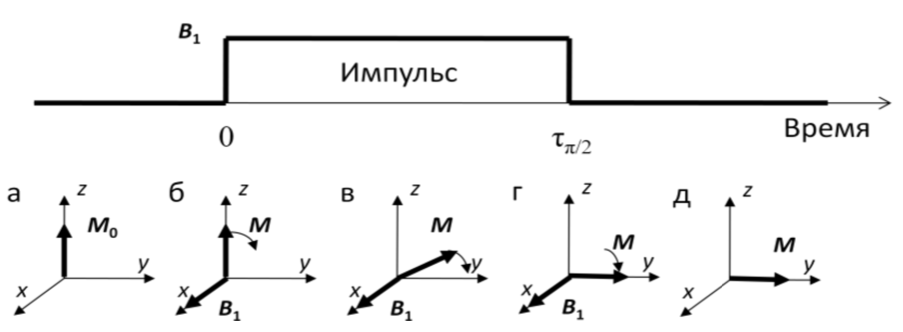
\includegraphics[scale = 0.3]{п:2 импульс.png}
    \caption{Поведение суммарной намагниченности под действием $\pi/2$-импульса (вращающаяся СК). A. до включения.Б. начало действия импульса.В. поворот намагниченности.г. окончание действия импульса.Д.прецессия намагниченности вокруг оси z после выключения импульса}
    \label{fig0}
\end{figure}



\subsection{Релаксация ядерной намагниченности}
Релаксация намагниченности - это процесс восстановления суммарной намагниченности к исходному равновесному состоянию. Уравнение Блоха с учетом процессов релаксации:

\begin{equation*}
    \frac{dM_z(t)}{dt} = \gamma [M_y B_z - M_z B_y] - \frac{M_z}{T_2} 
\end{equation*}

\begin{equation*}
    \frac{dM_y(t)}{dt} = \gamma [M_z B_x - M_x B_z] - \frac{M_y}{T_2} 
\end{equation*}  
    
\begin{equation*}
    \frac{dM_z(t)}{dt} = \gamma [M_x B_y - M_y B_x] - \frac{M_z - M_0}{T_1}
\end{equation*}
Решение уравнения Блоха после окончания действия $\pi/2$-импульса выглядит следующим образом:

\begin{equation*}
M(t) = M_0\begin{pmatrix}0\\e^\frac{-t}{T_2}\\1 - e^{\frac{-t}{T_1}} \end{pmatrix}
\end{equation*}

\subsection{Механизмы ЯМР-релаксации}
При тепловом движении частиц, имеющих магнитные моменты, возникают локальные магнитные поля, изменяющиеся во времени случайным образом. В спектре их случайных функций поля есть компоненты с частотой ЯМР. Их действие аналогично действию внешнего радиочастотного поля, т.е. переменное локальное поле может вызывать переходы между уровнями энергии спиновой системы. Изменяющееся случайным образом поле B′(t) можно описать с помощью корреляционной
функции K($\tau$):

\begin{equation*}
    K_i(\tau) = \overline{(B_i'(t) B_i'(t+\tau)}
\end{equation*}

где $B_i′$ – одна из компонент флуктуирующего поля, а черта означает усреднение по всевозможным реализациям этого произведения по различным начальным моментам времени t. Значения случайной функции на больших интервалах времени не коррелированы, следовательно, K при стремлении аргумента к бесконечности стремится к 0.

\item Поперечная релаксация определяется:
1. Компонентами локального поля, изменяющимися с частотами близкими к резонансной – аналогично спин-решеточной релаксации (спиновая подсистема отдает часть энергии термостату, потом берет обратно)
2. Потерей когерентности прецессии («сбой фазы прецессии») магнитных моментов, образующих вектор намагниченности  M из-за изменения частоты ЯМР в переменном поле B(t).

Выражение для скорости поперечной релаксации для системы невзаимодействующих друг с другом спинов в модели невзаимодействующих протонов в изотропном флуктуирующем локальном поле имеет вид:
\begin{equation*}
   \frac{1}{T_2} = \frac{1}{2T_1} + \frac{1}{T_2'} = \gamma\overline{|{B'(t)}|^2} (\frac{1}{2}J(w_0) + \frac{1}{2}J(0)) =\gamma^2\overline{|{B'(t)}|^2}(\frac{\tau_c}{1+w_0^2\tau_c^2} + \tau_c)
\end{equation*}

Во многих практически важных случаях K имеет вид:

\begin{equation*}
K(\tau) = \overline{|{B'(t)}|}^2 \exp^\frac{|{\tau}|}{\tau_C}
\end{equation*}

Спектральная плотность определяется как Фурье-преобразование функции корреляции:

\begin{equation*}
J(w) = \int_{+\infty}^{-\infty} K(\tau)\exp^{-iwt} \,d\tau \
\end{equation*}

Для нашей экспоненциальной функции:

\begin{equation*}
J(w) = \frac{2\tau_C}{1+w^2 \tau_c^2}\overline{|{B'(t)}|^2}
\end{equation*}

Поперечные компоненты локального флуктурирующего поля, направленные вдоль осей x и y и осциллирующие с резонансной частотой w0, приводят к спин-решеточной релаксации. Скорость продольной релаксации определяется J на частоте резонанса:

\begin{equation*}
\frac{1}{T_1} = \gamma^2 J(w_0) = \gamma^2\overline{|{B'(t)}|^2}\frac{2\tau_C}{1+w_0^2\tau_C^2}
\end{equation*}

\subsection{Импульсные последовательности. Последовательность КПМГ для регистрации времени $T_2$ и последовательность насыщение–восстановление для регистрации времен $T_1$}

Практически все современные методики использования ЯМР заключаются в изучении поведе-
ния намагниченности системы спинов после воздействия на нее определенной последовательности
радиочастотных импульсов. Простейшим примером является последовательность, состоящая из
одного $\pi/2$-импульса. После окончания действия радиочастотного импульса
зависимость поперечной намагниченности от времени во вращающейся системе координат будет определяться соотношением $M_y = M_0 exp^{-\frac{t}{T_2}}$. В ЛСО временная зависимость поперечной намагниченности  будет иметь вид $M_y' = M_0 exp^{-\frac{t}{T_2}}\sin{w_0t}$.

\begin{figure}[h!]
    \centering
    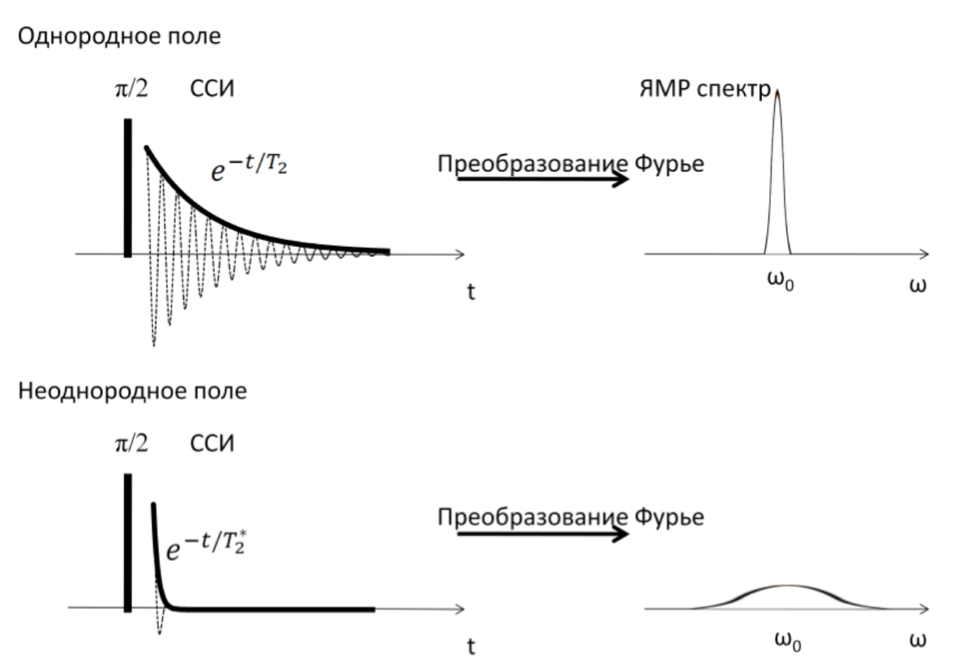
\includegraphics[scale = 0.3]{фурье.png}
    \caption{Спад свободной индукции после воздействия $\pi/2$-импульса в однородном и неоднородном магнитных полях}
    \label{fig0}
\end{figure}

Данную зависимость, регистрируемую после воздействия $\pi/2$-импульса, называют сигналом спада свободной индукции (ССИ). Фурье-преобразование зависимости $M_y′(t)$ позволяет получить частотный спектр ЯМР. В условиях реального эксперимента постоянное магнитное поле не является идеально однородным в объеме образца. Неоднородность поля приводит к тому, что прецессия векторов намагниченности происходит с разными частотами в разных областях пространства. Поэтому со временем фазовая когерентность прецессии векторов намагниченности разных частей образца теряется, в результате поперечная компонента суммарной намагниченности образца уменьшается. Общая скорость уменьшения поперечной намагниченности $(1/T_2^{*})$, фигурирующая в уравнении Блоха, в неоднородном магнитном поле определяется скоростью поперечной релаксации и потерей фазовой когерентности из-за неоднородности постоянного магнитного поля:

\begin{equation*}
\frac{1}{T_2^*} = \frac{1}{T_2} + \frac{\gamma\triangle B}{2}
\end{equation*}

 где $\triangle$ B характеризует неоднородность МП. Итак, если магнитное поле неоднородно, то регистри- ровать спектры ЯМР становится невозможно из-за значительного уширения сигналов. Анализ спада свободной индукции после воздействия $\pi/2$-импульса в таком поле не даст определить значение $T_2$. Для обхода этой проблемы используются специальные импульсные последовательности, основанные на явлении спинового эха Хартмана-Ханна.

 \begin{itemize}

 \item Для регистрации времен поперечной релаксации используется последовательность КПМГ. Импульсная последовательность КПМГ состоит из одного $\pi/2$ импульса, поворачивающего намагниченность на угол $\pi/2$ вокруг оси x, и серии $\pi$-импульсов, поворачивающих намагничен- ность на угол $\pi$ вокруг оси y, прикладываемых через определенные промежутки времени (рис. 3). Данная импульсная последовательность основана на наблюдении серии сигналов спинового эха Хартмана–Ханна. В отсутствие процессов поперечной релаксации амплитуда сигналов эха оставалась бы неизменной, а при протекании поперечной релаксации их амплитуда постепенно уменьшается. Время поперечной релаксации $T_2$ определяют из зависимости значения амплитуды сигнала эха M от времени между импульсами $\tau$ и номера сигнала эха n:
 
 \begin{equation*}
 M(2n\tau) = M_0 \exp^\frac{-2n\tau}{T_2}
\end{equation*}

Время $\tau$ обычно выбирается так, чтобы $\tau$ << $T_1$, восстановлением продольной компоненты намагниченности при этом можно пренебречь.

\item Для регистрации времен продольной релаксации используется импульсная последовательность насыщение–восстановление. Эта последовательность состоит из двух радиочастотных $\pi/2$- импульсов. До воздействия первого $\pi/2$ импульса, суммарная намагниченность $M_0$ системы ядер ориентирована параллельно оси z, направление которой совпадает с направлением постоянного магнитного поля $B_0$ (рис. а). Воздействуя в момент времени $\tau_1$ вторым $\pi/2$-импульсом, можно перевести продольную компоненту намагниченности $M_||$ в плоскость (x, y), в которой она может быть измерена (рис. г). После восстановления равновесия (в течение времени около $5T_1$) данную последовательность повторяют с увеличенным значением интервала между импульсами $\tau_1$. Время продольной релаксации $T_1$ определяют по зависимости значения $M||$ от времени между импульсами $\tau_1$ в серии экспериментов с различными значениями $\tau_1$:

\begin{equation*}
M_||(\tau_1) = M_0( 1 - exp^\frac{\tau_1}{T_1})
\end{equation*}

\begin{figure}[h!]
    \centering
    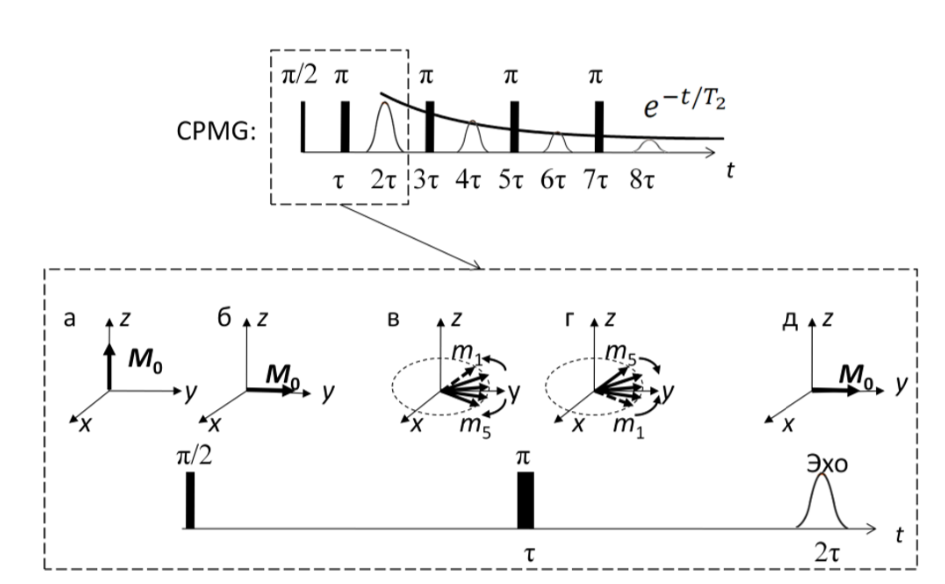
\includegraphics[scale = 0.3]{кпмг.png}
    \caption{Импульсная последовательность КПМГ, используемая для регистрации времѐн поперечной релаксации T2}
    \label{fig0}
\end{figure}

 \end{itemize}

\newpage
\section{Экспериментальная установка}

\textbf{Используемые приборы и материалы:}
\begin{itemize}

\item ЯМР-релаксометр Bruker Minispec.

\item Исследуемые вещества: $\text{H}_2\text{O}$; $\text{MnSO}_4$, $C_{\text{соли}}=0.25M$; $\text{Na}_2\text{SO}_4$, $C_{\text{соли}} = 0.25M$.

\end{itemize}


\begin{figure}[h!]
    \centering
    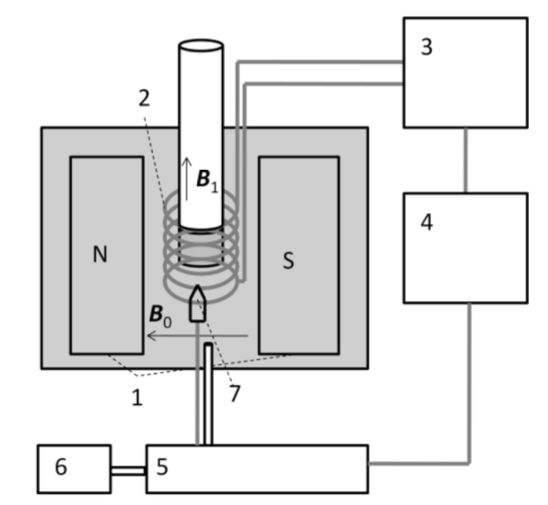
\includegraphics[scale = 0.4]{схема.png}
    \caption{Принципиальная схема ЯМР-релаксометра: 1 – постоянный магнит, 2 – приемо-передающая катушка, 3 – генератор импульсов и приемник излучения, 4 – компьютер, 5 – система термостатирования образца, 6 – воздушный компрессор, 7 – термопара}
    \label{fig0}
\end{figure}

Основной частью ЯМР-релаксометра является магнит (1 на рис. 4), создающий постоянное магнитное поле напряженностью B0. Величина напряженности постоянного МП релаксометра Bruker minispec, используемого в этой работе, составляет около 0.5 Тл (5 · 103 Гс). Этой напряженности соответствует рабочая частота для протонов B0 = 20 МГц. 
	Переменное магнитное поле, перпендикулярное постоянному магнитному полю, создается при помощи катушки индуктивности, вдоль оси которой располагается пробирка с исследуемым образцом. Параллельно катушке включен конденсатор так, что образованный радиочастотный контур настроен на резонансную ларморовскую частоту. 
Для создания импульсов переменного поля катушка 2 соединяется с радиочастотным генератором, расположенным в 3. Слабый сигнал ЯМР предварительно усиливается, затем поступает в блок управляющей электроники, где и производится его детектирование. При этом следует учитывать наличие переходных процессов в приемном контуре и усилителе, из-за которых у приемника существует т.н. «мертвое время» порядка 100 нс, необходимое для переключения в режим приема и усиления слабого сигнала намагниченности после периода генерации мощных импульсов. 





\newpage

\section{Ход работы и обработка результатов}

\subsection{Определение длительности $\pi/2$ и $\pi$ импульсов}

\textbf{\textit{Задание:}} Постройте зависимость амплитуды намагниченности от длительности радиочастотного импульса. Определите по графику длительности $90^\circ$ и $180^\circ$ импульсов.

\begin{itemize}


 \item Для проведения данного эксперимента использовалась программа pulses10MHz программного обеспечения ЯМР-релаксометра, которая измеряет амплитуду сигнала FID $\sim M_x$ в зависимости от времени.

  \item  Согласно теории, угол поворота вектора намагниченности от равновесного положения (параллельного z) $\theta=\gamma B_1 \tau_\theta$, где $B_1 ~ sin(wt)$ - вращающееся в плоскости xy переменное магнитное поле, $\tau_\theta$ - длительность импульса. Проекция вектора намагниченности, повернутоно на угол $\theta$ относительно z: $M_x \sim sin(\theta) \sim sin(\gamma B_1 \tau_\theta)$. Значит, экспериментальные данные должны описываться синусоидальной зависимостью.

\begin{figure}[h!]
    \centering
    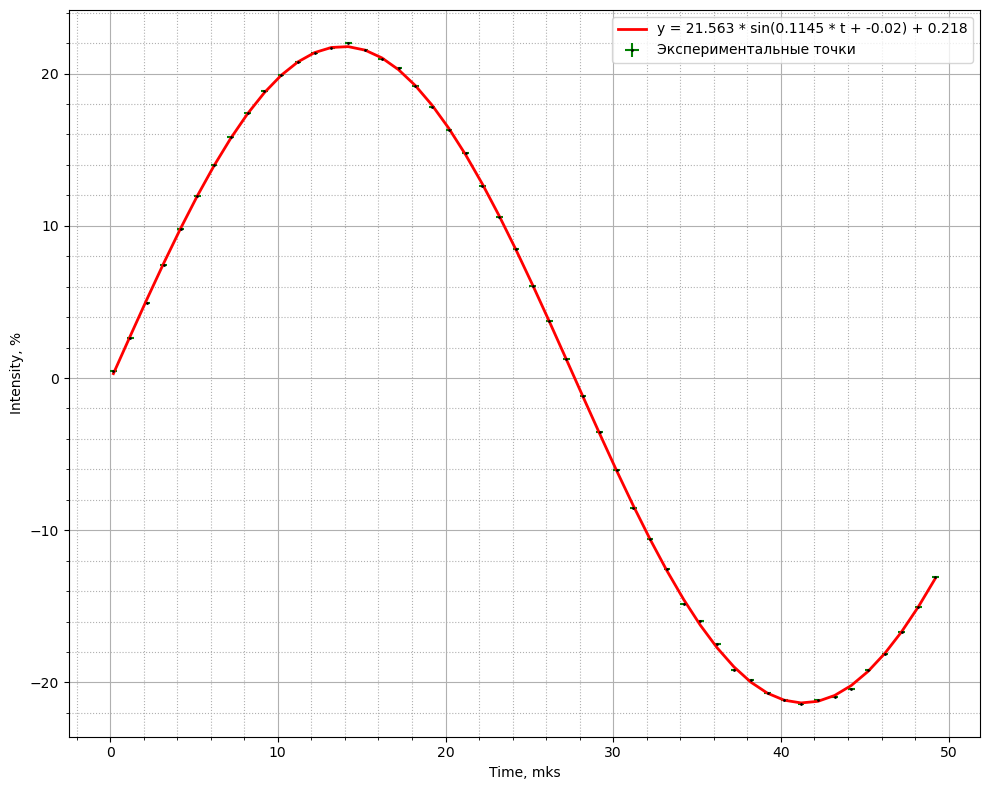
\includegraphics[scale = 0.4]{graphs/sin.png}
    \caption{Зависимость амплитуды намагниченности $M_x$ от длительности сигнала}
    \label{sin}
\end{figure}

\item Полученные данные (\hyperref[sin]{Рисунок \ref*{sin}}) с хорошей точностью описываются функцией $y=A \cdot \sin(\omega \cdot t + \phi)$. Отсюда можно найти длительности $\pi/2 $ и $\pi$ импульсов: когда $(\omega \cdot t + \phi )=\pi /2 $,  проекция вектора намагниченности на ось х максимальна, а $(\omega \cdot t + \phi )=\pi$, она равна нулю. 

\item После построоения графика и аппроксимации данных синусоидой, получаем: 
\begin{equation*}
    \tau_{90} = (13.4\pm 1.4) \text{мкс}, ~~~
    \tau_{180} = (27.6\pm 2.8)\text{мкс}
\end{equation*}

\end{itemize}

\subsection{Оценка скорости релаксации воды} 
\label{relax}

\subsubsection{Оценка времени поперечной релаксации воды $T_2$}\label{t2}


\textbf{\textit{Задание:}} Постройте график зависимости амплитуды сигнала эха от времени для образца, состоящего из воды, используя экспериментальные данные, полученные при измерении $T_2$. Определите по графику значение времени $T_2$ воды.

\begin{itemize}

\item Для нахождения времени поперечной релаксации $T_2$ используется последовательность импульсов КПМГ. В данном эксперименте для заданния такой импульсной последовательности использовалось приложение t2\_cpmg.app. 

\item Из теоретического введения известно, что амплитуда сигнала эха для КПМГ зависит от времени (т.е. от номера сигнала и временем между импульсами) как $M(t) \sim e^{-t/T_2}$. 

\begin{figure}[h!]
    \centering
    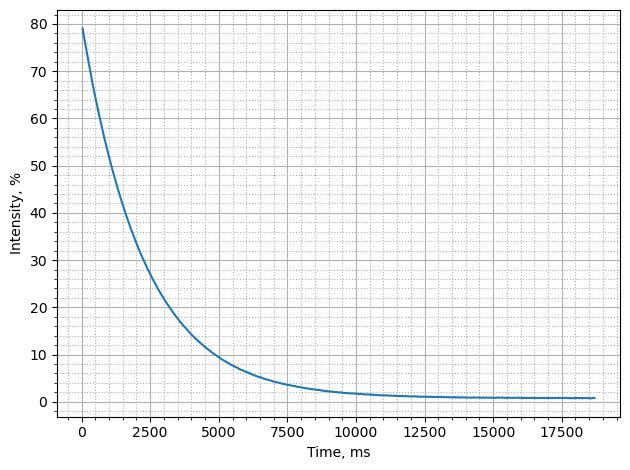
\includegraphics[scale = 0.7]{graphs/cmpg_h20.png}
    \caption{Экспериментальная зависимость амплитуды сигнала эха импульсной последовательности КПМГ для воды}
    \label{h2o}
\end{figure}

\item Для получения значения $T_2$ построим полученную зависимость (\hyperref[h20]{Рисунок \ref*{h2o}}) в логарифмических координатах (\hyperref[h2o_log]{Рисунок \ref*{h2o_log}}). Тогда из угла наклона прямой, проведенной по точкам до изгибания кривой получаем $T_2(H_2O)=(2396\pm4)$ мс.



\begin{figure}[h!]
    \centering
    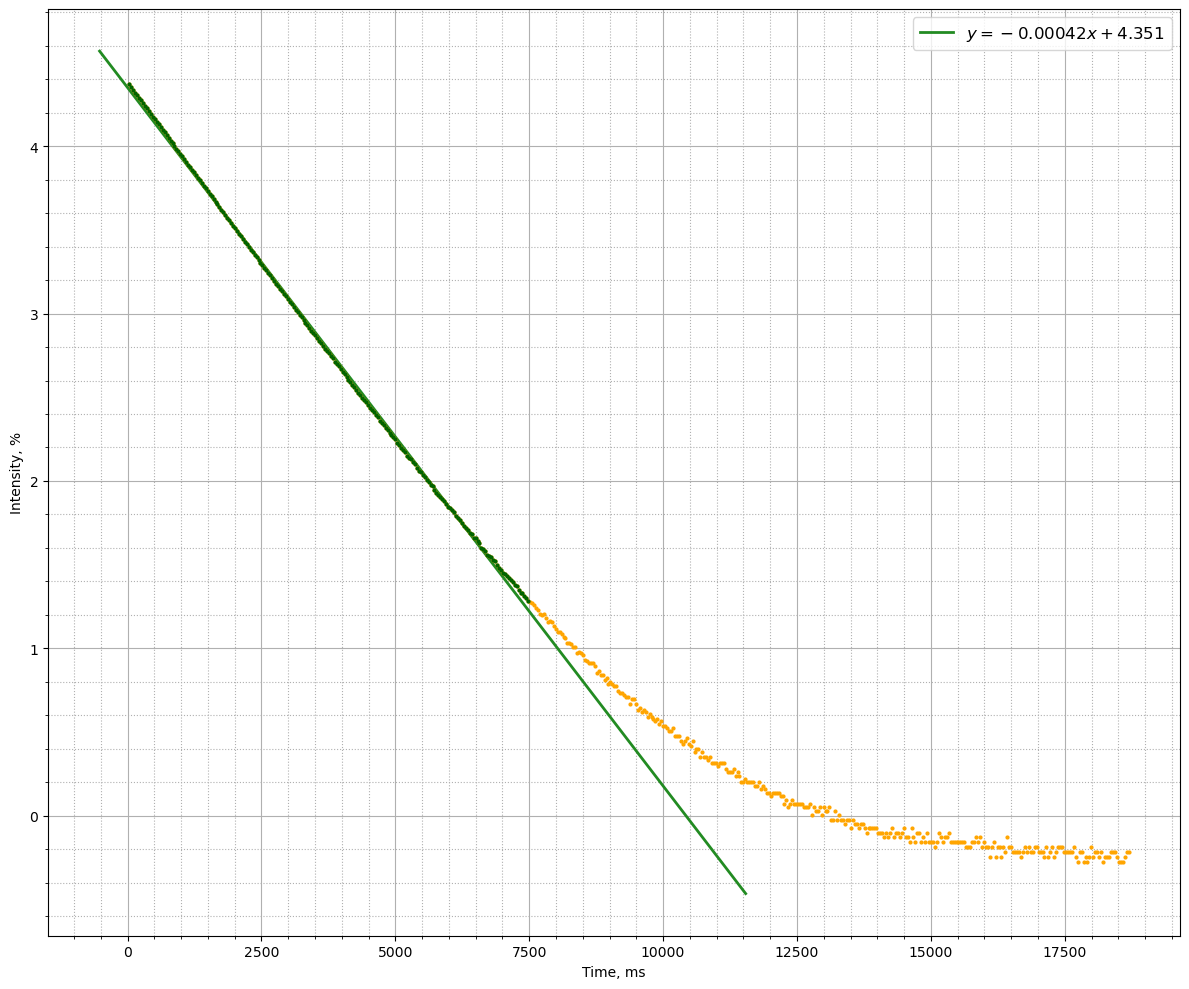
\includegraphics[scale = 0.4]{graphs/cmpg_h2o_log.png}
    \caption{Зависимость амплитуды сигнала эха импульсной последовательности КПМГ для воды в логарифмических координатах}
    \label{h2o_log}
\end{figure}


\end{itemize}


\subsubsection{Оценка времени продольной релаксации воды $T_1$} \label{t1}
\textbf{\textit{Задание:}} Постройте график зависимости амплитуды намагниченности от времени для образца, состоящего из воды, используя экспериментальные данные, полученные при измерении $T_1$. Определите по графику значение времени $T_1$ воды
\\ \par

\begin{itemize}

\item Для нахождения времени продольной релаксации $T_1$ используется последовательность импульсов 'насыщение-восстановление', реализуемая в данном эксперименте с помощью програмы «t1\_saturation \_recovery.app».
\item Из теоретического введения известно, что амплитуда сигнала эха для 'насыщение-восстановления' зависит от времени как $M(t) \sim 1-e^{-t/T_1}$ 

\begin{figure}[h!] \label{fig4}
    \centering
    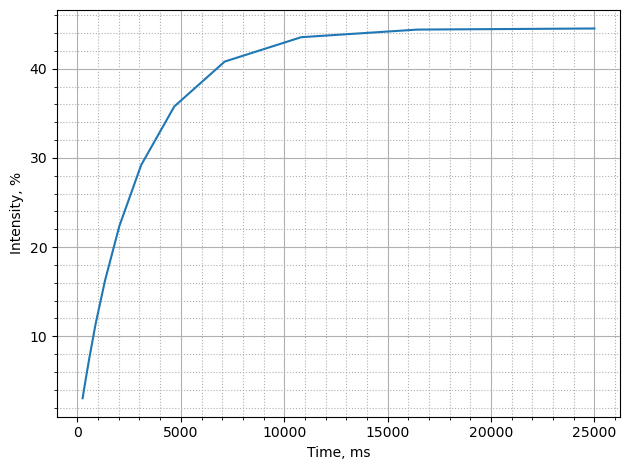
\includegraphics[scale = 0.7]{graphs/h20_t1.png}
    \caption{Экспериментальная зависимость амплитуды сигнала импульсной последовательности 'насыщение-восстановление' для воды}
    \label{h2o_t1}
\end{figure} 

\item Для получения значения $T_1$  сделаем аппроксимацию полученных даных (\hyperref[h2o_t1]{Рисунок \ref*{h2o_t1}}) нашей теоретической зависимостью(\hyperref[h2o_t1_app]{Рисунок \ref*{h2o_t1_app}}), в результате получаем: $T_1=(2940\pm 35)ms$.


\begin{figure}[h!] \label{fig4}
    \centering
    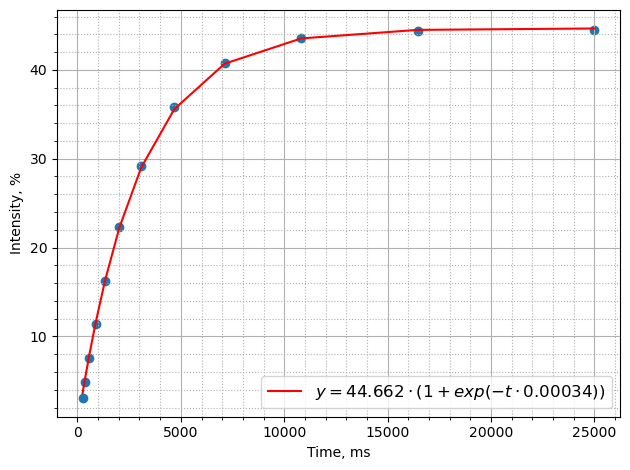
\includegraphics[scale = 0.7]{graphs/t1_h2o_approx.png}
    \caption{ Аппроксимация зависимости амплитуды сигнала импульсной последовательности 'насыщение-восстановление' для воды}
    \label{h2o_t1_app}
    
\end{figure}

\end{itemize}


\subsubsection{Оценка времени спада свободной индукции воды $T_2^*$}

\textbf{\textit{Задание:}} Постройте спад свободной индукции для образца, состоящего из воды, используя экспериментальные данные, полученные при измерении $T_2^*$. Определите по графику значение времени $T_2^*$ воды.
\\ \par
\begin{itemize}


\item Спад свободной индуции - это временная зависимость поперечной компоненты намагниченности после воздействия одиночного $\pi/2$ импульса.

\item Из решения уравнения Блоха в лабораторной системе отсчета $M_y \sim e^{-t/T_2^*}sin(w_0t)$, где $w_0$ - ларморовская частота $w_0=\gamma B_0$.

\begin{figure}[h!]
    \centering
    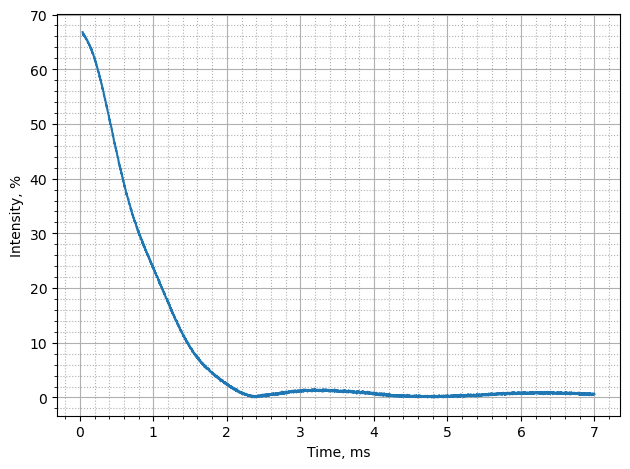
\includegraphics[scale = 0.7]{graphs/h2o_t2_selected.png}
    \caption{Экспериментальная зависимость спада свободной индукции воды после действия $\pi/2$ импульса}
    \label{h2o_t2_selected}
\end{figure}

\item  Для получения значения $T_2^{*}$ построим полученную зависимость (\hyperref[h2o_t2_selected]{Рисунок \ref*{h2o_t2_selected}}) в логарифмических координатах (\hyperref[h2o_t2_selected_log]{Рисунок \ref*{h2o_t2_selected_log}}). Тогда из угла наклона прямой, проведенной по точкам до изгибания кривой получаем $T_2^{*}(H_2O)=(0.7782\pm0.0010)$ мс.


\begin{figure}[h!]
    \centering
    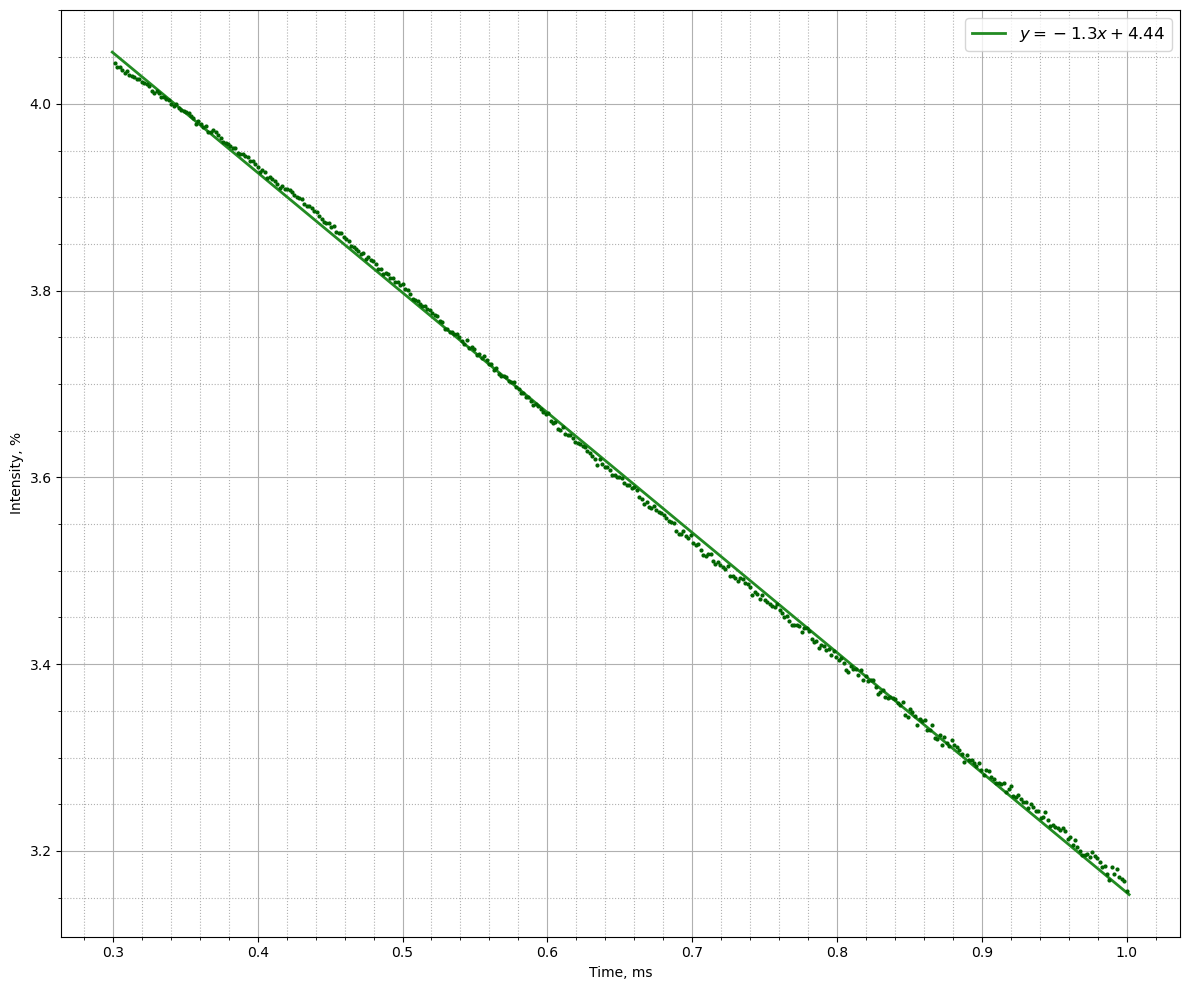
\includegraphics[scale = 0.3]{graphs/h2o_t2_selected_app.png}
    \caption{Аппроксимация зависимости спада свободной индукции воды после действия $\pi/2$ импульса в логарифмических координатах}
    \label{h2o_t2_selected_log}
\end{figure}


\end{itemize}


\subsubsection{Оценка неоднородности постоянного магнитного поля $B_0$}
\begin{itemize}

\item Полная скорость уменьшения поперечной намагниченности состоит из скорости поперечной релаксации и и потерей фазовой когерентности из-за неоднородности 
постоянного магнитного поля ($\Delta B_0$ - неоднородность постоянного магнитного поля)
\begin{equation*}
    \frac{1}{T_2^*} = \frac{1}{T_2}+\frac{\gamma \Delta B_0}{2}
\end{equation*}

\begin{equation*}
    \Delta B_0 = \frac{2}{\gamma}\left( \frac{1}{T_2^*}-\frac{1}{T_2} \right), ~~~ \sigma \Delta B_0 = \frac{2}{\gamma}\sqrt{\left(\frac{\sigma T_2^*}{T_2^*^2}\right)^2+\left(\frac{\sigma T_2}{T_2^2}\right)^2}
\end{equation*}
\item В воде присутствуют атомы H и O, при этом ЯМР может наблюдаться на $H^+$ (т.к. у $O^{2-}$ полная внешняя 2p оболочка, суммарный спин 0, т.е. это диамагнитный атом). Гиромагнитное соотношение для протона (g=5.585) $\gamma = g\cdot \gamma_0 =42.58 $МГц/Тл
\begin{equation*}
    \Delta B_0 = (60.34 \pm 0.10)\text{мкТл}
\end{equation*}
\item Из сведений об экспериментальной установке $B_0\approx 0.5$Тл. Значит, $\Delta B_0 << B_0$, то есть магнитное поле действительно постоянное.

\end{itemize}



\subsection{Оценка скорости релаксации в растворах $MnSO_4$ и $Na_2SO_4$ различной концентрации}


\textbf{\textit{Задание:}} Постройте зависимости скоростей продольной и поперечной релаксации (1/$T_1$, 1/$T_2$ и 1/$T_2^*$) от концентрации солей сульфатов. Объясните различия в зависимостях скоростей релаксации для различных сульфатов.

\begin{itemize}


\item Приготовим растворы солей в воде объемом $V_{\text{воды}}=(33.0 \pm0.5)$мл. Добавим  по $V=(10.0\pm 0.5)$мкл растворов MnSO4 ($C_{соли}=0.25M)$ и Na\_2SO4($C_{соли} = 0.25M$) в пробирку с водой. Концентрация соли C в растворах считаем по формуле:
\begin{equation*}
    C = \frac{C_{\text{соли}}V_{\text{соли}}}{V_{\text{соли}}+V_{\text{воды}}}
\end{equation*}

\item На \hyperref[gather_t2]{Рисунок \ref*{gather_t2}}, \hyperref[gather_t1]{Рисунок \ref*{gather_t1}} показаны результаты снятия релаксационных кривых для солей различных концентраций. Для образца $MnSO_4$, 40 мкл не была получена зависимость амплитуды сигнала эха импульсной
последовательности КМПГ для
определения $T_2$.


\begin{figure}[h!]
\begin{minipage}[h]{0.49\linewidth}
\center{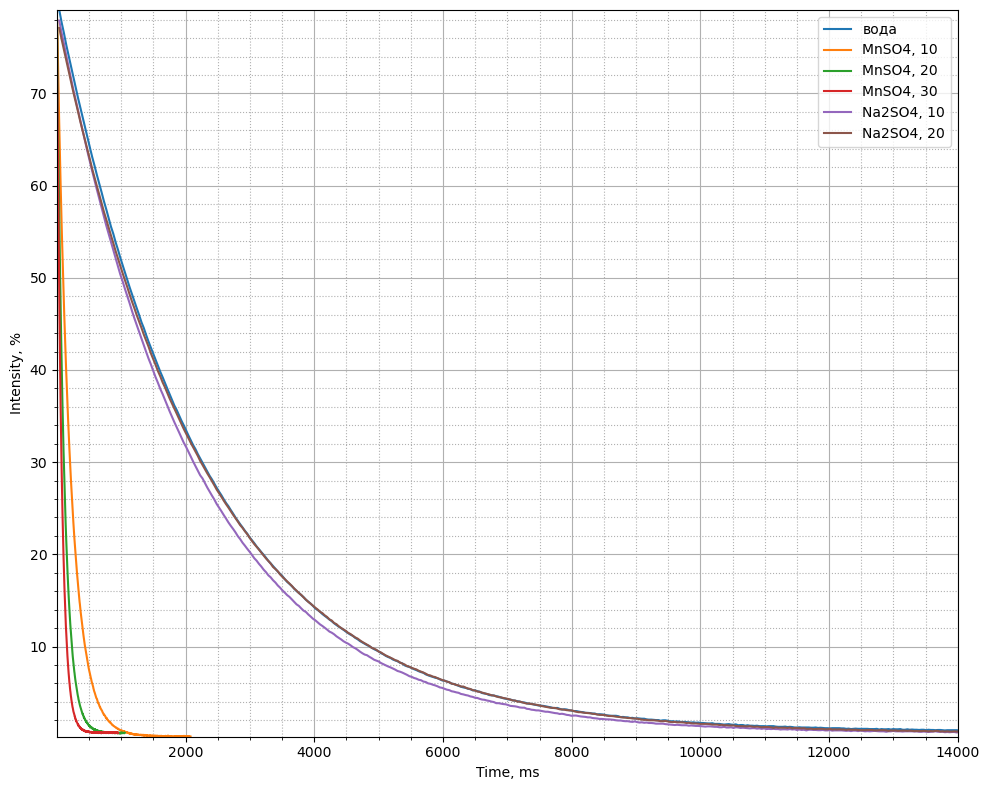
\includegraphics[width=1\linewidth]{graphs/gather_t2.png}} \caption{Экспериментальная зависимость амплитуды сигнала эха импульсной последовательности КПМП для определения $T_2$} \label{gather_t2} \\

\end{minipage}
\hfill
\begin{minipage}[h]{0.49\linewidth}
\center{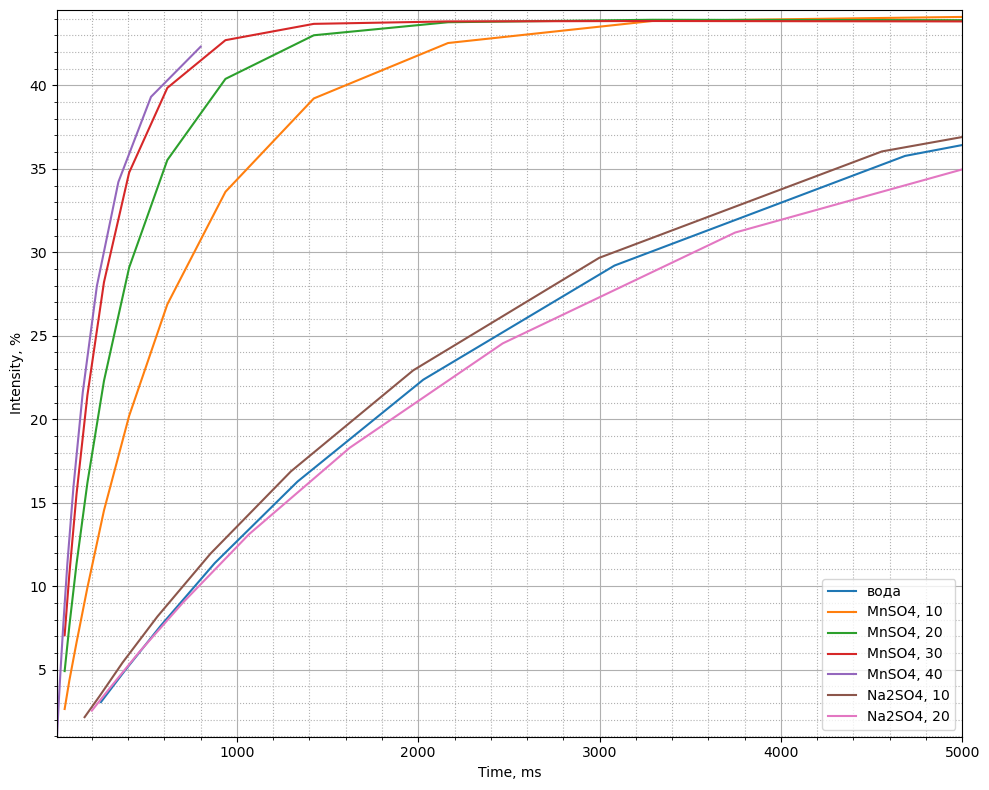
\includegraphics[width=1\linewidth]{graphs/gather_t1.png}} \caption{Экспериментальная зависимость амплитуды сигнала эха импульсной последовательности saturation-recovery для определения $T_1$}\label{gather_t1} \\
\end{minipage}
\end{figure} 


\item Проведем расчеты значений скоростей релаксации исследуемых растворов аналогично тем, что мы провели для воды(\hyperref[tab:my-table]{Таблица \ref*{tab:my-table}}).

\begin{table}[h!]
\label{table}
\centering
\caption{Сводная таблица результатов измерений времен релаксации для растворов солей различных концентраций }
\begin{tabular}{|c|c|cccc|cc}
\hline
 &
  вода 33 мл &
  \multicolumn{4}{c|}{раствор MnSO4 (0.25М)} &
  \multicolumn{2}{c}{раствор $Na_2SO4$ (0.25M)} \\ \hline
Vсоли, мкл &
  0 &
  \multicolumn{1}{c|}{10} &
  \multicolumn{1}{c|}{20} &
  \multicolumn{1}{c|}{30} &
  40 &
  \multicolumn{1}{c|}{10} &
  \multicolumn{1}{c|}{20} \\ \hline
С(соли), мкM &
  0 &
  \multicolumn{1}{c|}{76} &
  \multicolumn{1}{c|}{151} &
  \multicolumn{1}{c|}{227} &
  303 &
  \multicolumn{1}{c|}{76} &
  \multicolumn{1}{c|}{151} \\ \hline
\sigma C, $\text{мкМ}$ &
  0 &
  \multicolumn{1}{c|}{8} &
  \multicolumn{1}{c|}{8} &
  \multicolumn{1}{c|}{8} &
  8 &
  \multicolumn{1}{c|}{8} &
  \multicolumn{1}{c|}{8} \\ \hline
T2, ms &
  2396 &
  \multicolumn{1}{c|}{214.11} &
  \multicolumn{1}{c|}{117.0} &
  \multicolumn{1}{c|}{77.16} &
  - &
  \multicolumn{1}{c|}{2279} &
  \multicolumn{1}{c|}{2408} \\ \hline
\sigma T2, ms &
  4 &
  \multicolumn{1}{c|}{0.18} &
  \multicolumn{1}{c|}{0.2} &
  \multicolumn{1}{c|}{0.14} &
  - &
  \multicolumn{1}{c|}{4} &
  \multicolumn{1}{c|}{3} \\ \hline
T1, ms &
  2941 &
  \multicolumn{1}{c|}{668} &
  \multicolumn{1}{c|}{380} &
  \multicolumn{1}{c|}{262} &
  218 &
  \multicolumn{1}{c|}{2695} &
  \multicolumn{1}{c|}{2976} \\ \hline
\sigma T1, ms &
  34 &
  \multicolumn{1}{c|}{8} &
  \multicolumn{1}{c|}{3} &
  \multicolumn{1}{c|}{2} &
  3 &
  \multicolumn{1}{c|}{20} &
  \multicolumn{1}{c|}{18} \\ \hline
1/T2, \cdot 10^{6} ms^{-1} &
  417.4 &
  \multicolumn{1}{c|}{4670} &
  \multicolumn{1}{c|}{8547} &
  \multicolumn{1}{c|}{12960} &
  - &
  \multicolumn{1}{c|}{438.8} &
  \multicolumn{1}{c|}{415.3} \\ \hline
\sigma (1/T2), \cdot $10^{6}ms^{-1}$ &
  0.7 &
  \multicolumn{1}{c|}{4} &
  \multicolumn{1}{c|}{15} &
  \multicolumn{1}{c|}{20} &
  - &
  \multicolumn{1}{c|}{0.8} &
  \multicolumn{1}{c|}{0.5} \\ \hline
1/T1, \cdot 10^{4} ms^{-1} &
  3.4 &
  \multicolumn{1}{c|}{14.97} &
  \multicolumn{1}{c|}{26.32} &
  \multicolumn{1}{c|}{38.17} &
  45.87 &
  \multicolumn{1}{c|}{3.71} &
  \multicolumn{1}{c|}{3.36} \\ \hline
\sigma (1/T1), \cdot $10^{4}ms^{-1}$ &
  0.04 &
  \multicolumn{1}{c|}{0.18} &
  \multicolumn{1}{c|}{0.21} &
  \multicolumn{1}{c|}{0.29} &
  0.63 &
  \multicolumn{1}{c|}{0.03} &
  \multicolumn{1}{c|}{0.02} \\ \hline
\end{tabular}
\label{tab:my-table}
\end{table}


\begin{figure}[h!]
\begin{minipage}[h]{0.49\linewidth}
\center{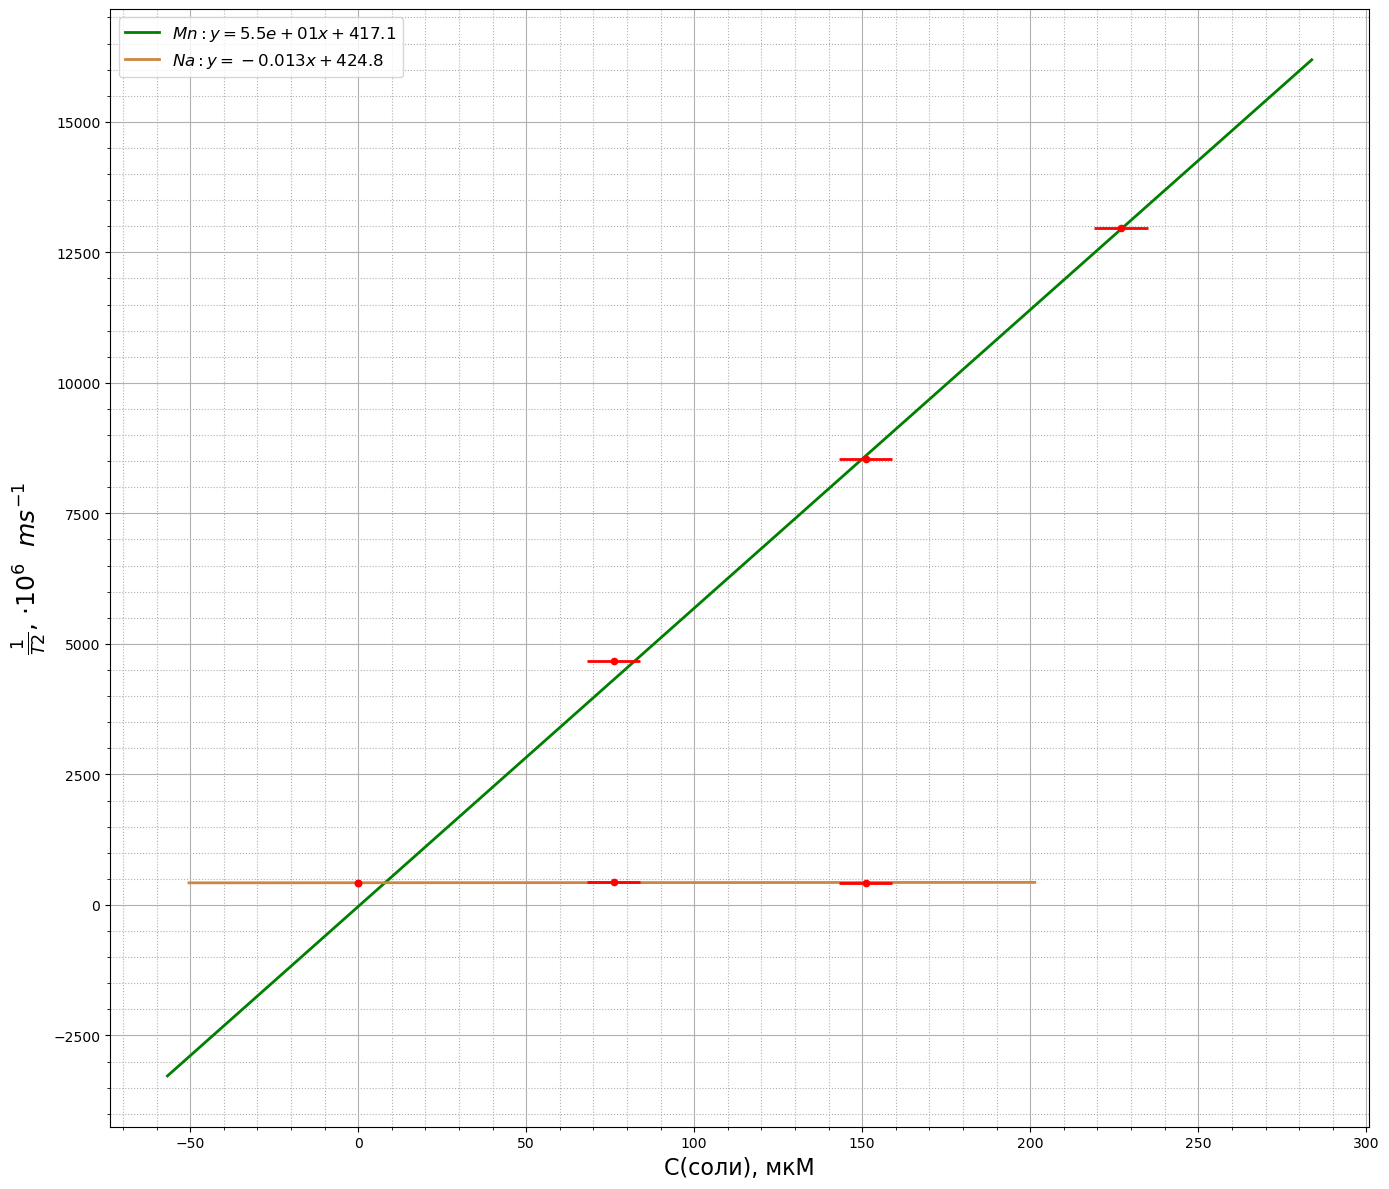
\includegraphics[width=1\linewidth]{graphs/one_t2.png}} \caption{Экспериментальная зависимость амплитуды сигнала эха импульсной последовательности КПМП для определения $T_2$} \label{one_t2} \\
\end{minipage}
\hfill
\begin{minipage}[h]{0.49\linewidth}
\center{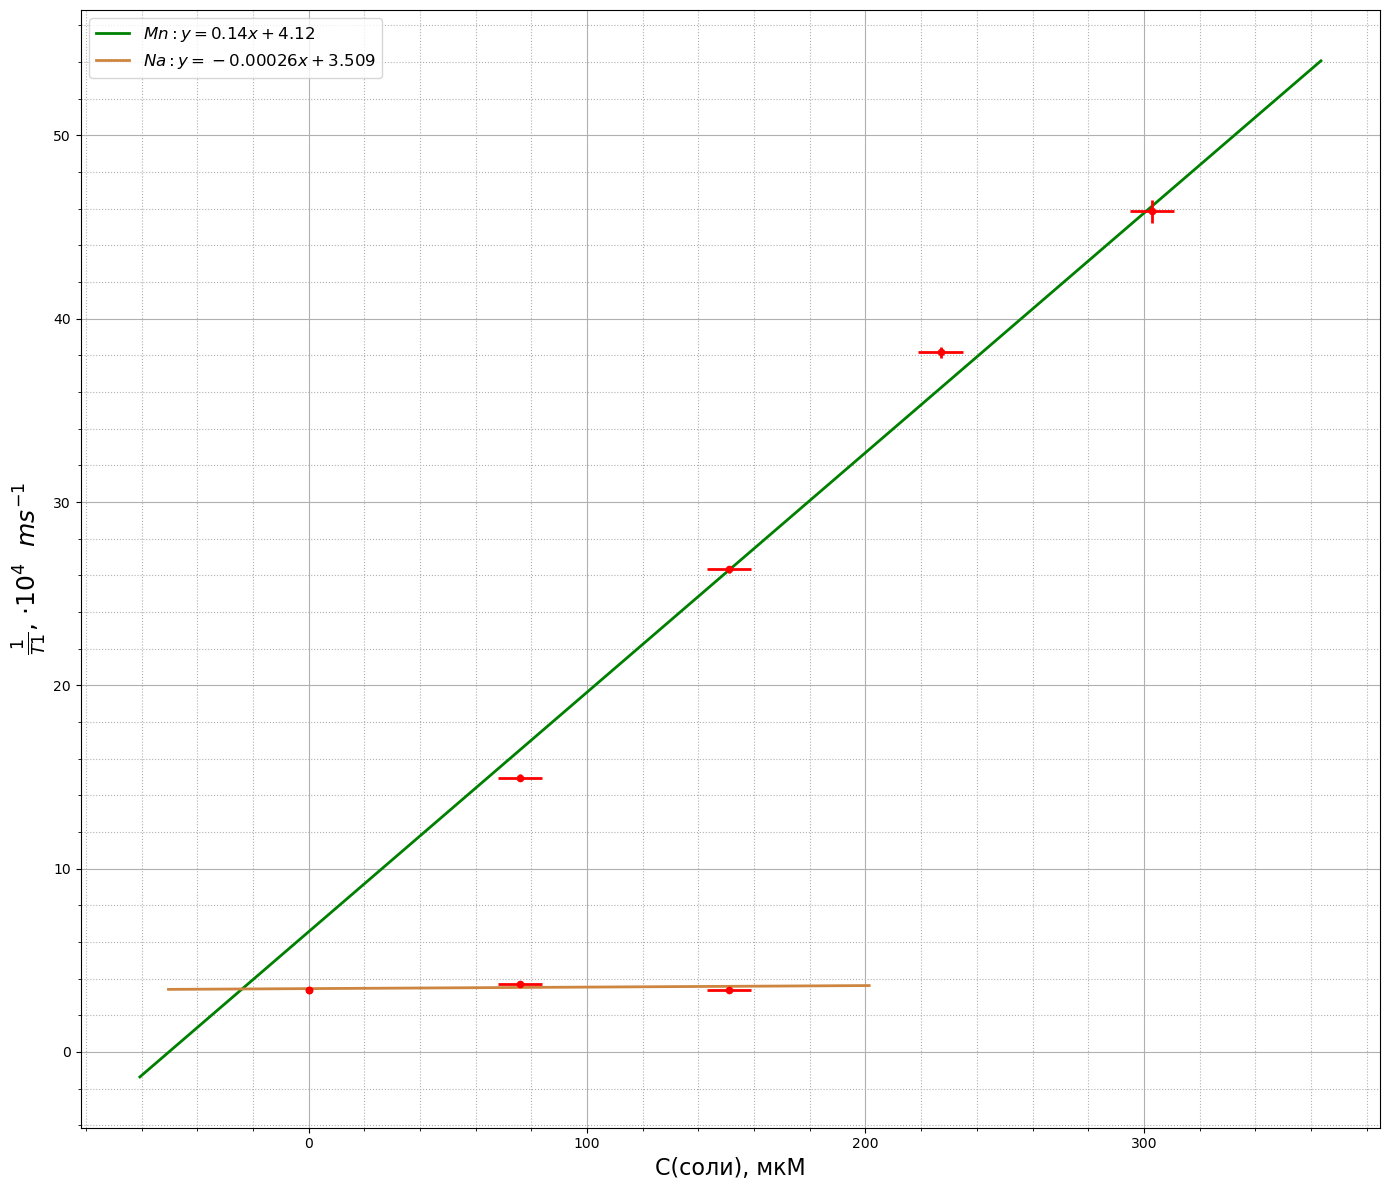
\includegraphics[width=1\linewidth]{graphs/one_t1.png}} \caption{Экспериментальная зависимость амплитуды сигнала эха импульсной последовательности saturation-recovery для определения $T_1$}\label{one_t1} \\
\end{minipage}
\end{figure} 


\item  Используя данные \hyperref[tab:my-table]{Таблицы \ref*{tab:my-table}}, построим зависимости скоростей продольной и поперечной релаксации (1/$T_1$, 1/$T_2$ и 1/$T_2^*$) от концентрации солей сульфатов (\hyperref[one_t2]{Рисунок \ref*{one_t2}}, \hyperref[one_t1]{Рисунок \ref*{one_t1}}).




\item
Из графиков \hyperref[one_t2]{Рисунка \ref*{one_t2}}, \hyperref[one_t1]{Рисунка \ref*{one_t1}} видно, что для $MnSO_4$ с увеличением концентрации соли скорость релаксации линейно увеличивается, в отличие от $Na_2SO_4$. Данный эффект объясняется тем, что $Mn^{2+}$ - парамагнитный ион (имеет неспаренные электроны на внешней электронной оболочке, т.е. обладает ненулевым магнитным моментом в отсутствии внешнего магнитного поля (см.рис. \ref{13}-\ref{14}).

\begin{figure}[h!]
\begin{minipage}[h]{0.5\linewidth}
\center{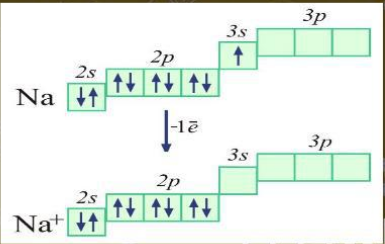
\includegraphics[width=0.7\linewidth]{el_conf_na.png}} \caption{ Электронное строение диамагнитного катиона $Na^+$} \label{13} \\
\end{minipage}
\hfill
\begin{minipage}[h]{0.5\linewidth}
\center{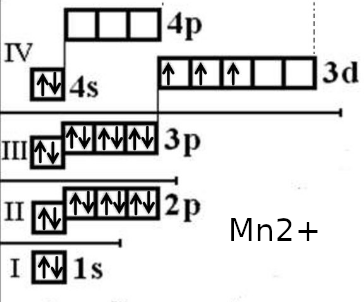
\includegraphics[width=0.7\linewidth]{el_cong_mn2+.png}} \caption{Электронное строение парамагнитного катиона $Mn^{2+}$} \label{14} \\
\end{minipage}
\end{figure} 



\item Согласно теории, скорость релаксации протонов в растворе с парамагнитными ионами растет пропорционально концентрации этих ионов: $\frac{1}{T_i} \sim [N], i = 1,2$. Это объясняется формированием вокруг парамагнитных ионов координационной сферы из воды,  скорость релаксации протонов в которой увеличена. Остальные протоны оказываются так же вовлечены во взаимодействие с неспаренными
электронами парамагнитных частиц за счет диффузии и обменных процессов между молекулами.\\

\item Таким образом, на \hyperref[one_t2]{Рисунках \ref*{one_t2}}, \hyperref[one_t1]{Рисунках \ref*{one_t1}} мы видим линейный рост скорости для парамагнитного иона и отсутсвие такого эффекта для диамагнитного иона, что хорошо объясняется теорией. 


\end{itemize}

\section{Выводы}


\begin{enumerate}
    \item Были определены длительности 90$\circ$ и 180$\circ$ импульсов: $\tau_{90} = (13.4\pm 1.4) \text{мкс}, $\tau_{180} = (27.6\pm 2.8)\text{мкс}$.
    
    \item Для воды было определено время $T_2(H_2O)=(2396\pm4)$ мс,  $T_1(H_2O)=(2940\pm 35)$ мс,  $T_2^{*}(H_2O)=(0.7782\pm0.0010)$ мс.
    
    \item При измерении скорости релаксации протонов в воде была оценена степень неоднородности постоянного магнитного поля. Оказалось, что поле практически однородно.
    
    \item Для всех образцов солей были определены значения  $T_1$, $T_2$ и $T_2^{*}$ (\hyperref[tab:my-table]{Таблица\ref*{tab:my-table}}).
    % \item  Из графиков зависимости скоростей релаксации (1/$T_1$, 1/$T_2$, 1/$T_2^*$) от концентрации соли была получена возрастающая зависимость, подтверждающая теоретические соображения. Опираясь на теорию, можно предсказать, что скорость релаксации сульфата марганца много больше скорости релаксации сульфата натрия в силу отсутствия спина у иона $Na^+$.
    \item  Из графиков зависимости скоростей релаксации (1/$T_1$, 1/$T_2$, 1/$T_2^*$) от концентрации соли была получена возрастающая зависимость. Эти экспериментальные данные показывают, что скорость релаксации намагниченности линейно возрастает для сульфатов парамагнитных ионов и практически не изменяется для диамагнитных. Этот эффект объясняется возникновением вокруг парамагнитных ионов координационной водной сферы, в которой скорость релаксации протонов увеличена. Остальные протоны так же вовлекаются во взаимодействие с неспаренными элетронами ионов за счет диффузии и обменных процессов между ионами.

\end{enumerate}


\end{document}